\chapter{Результат}

На рисунке \ref{fig:gui} представлен графический интерфейс приложения.

\begin{figure}[H]
	\centering
	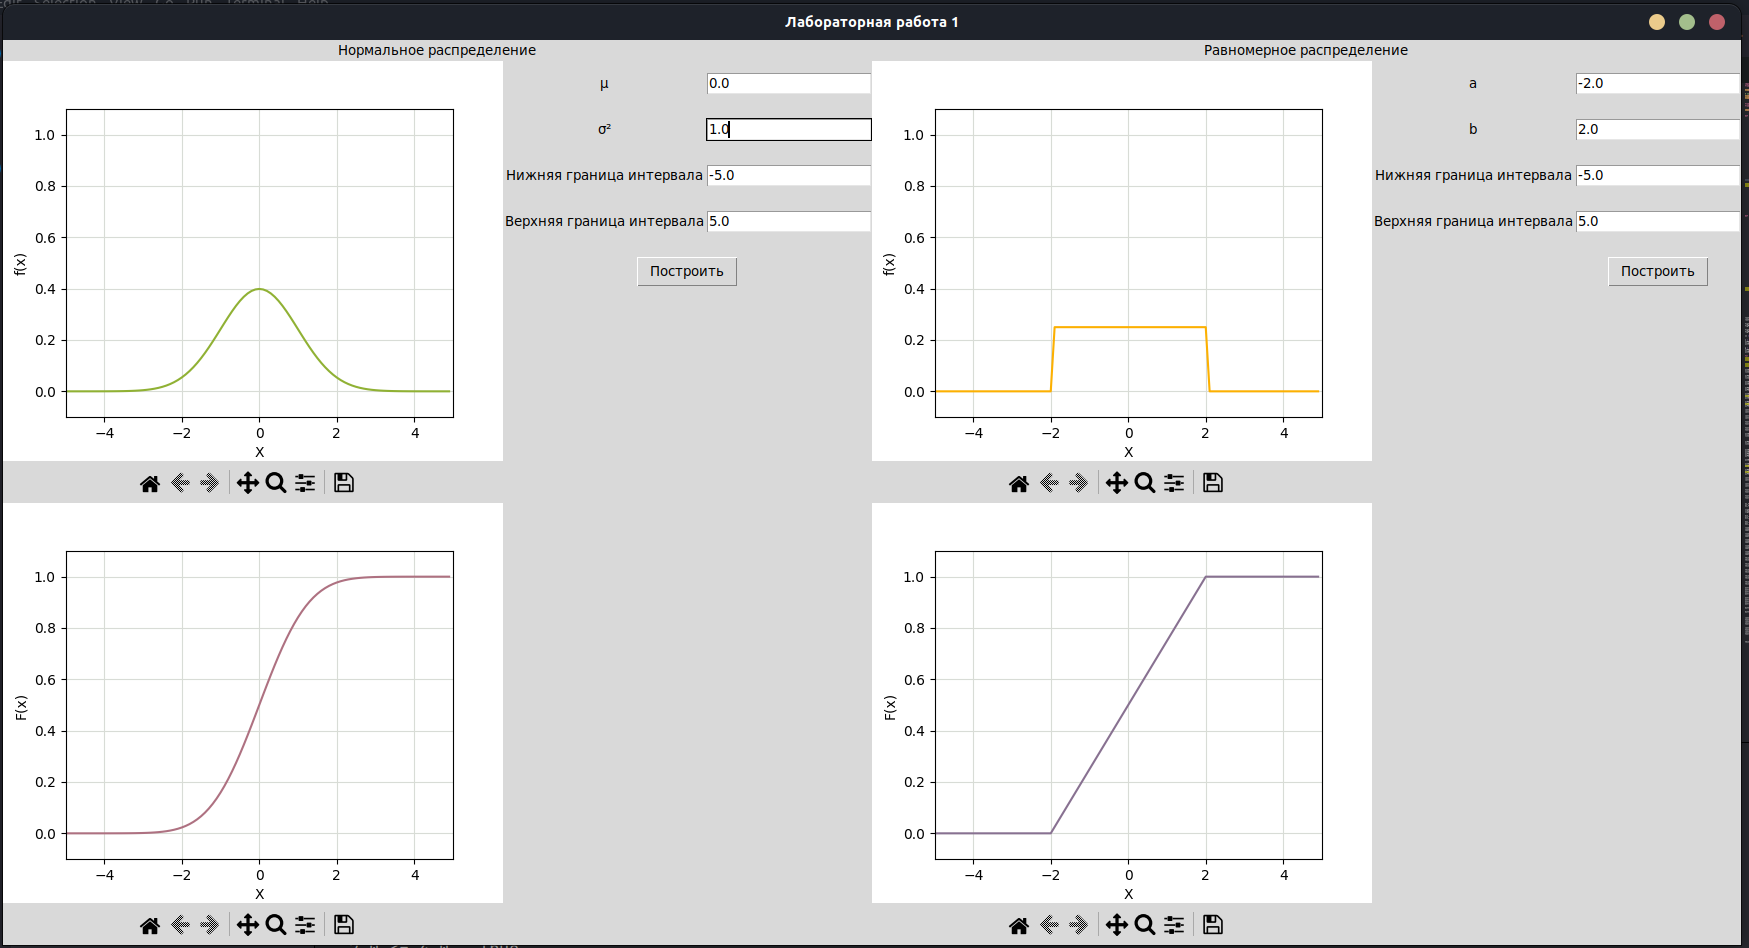
\includegraphics[width=\linewidth]{assets/gui.png}
	\caption{Графический интерфейс приложения}
	\label{fig:gui}
\end{figure}

Если пользователь ввёл некорректные данные, он увидит предупреждение с ошибкой и названием поля с некорректными данными (рисунок \ref{fig:msgbox}).

\begin{figure}[H]
	\centering
	
\includegraphics[width=0.6\linewidth]{assets/msgbox.png}
	\caption{Графический интерфейс приложения}
	\label{fig:msgbox}
\end{figure}

На рисунках \ref{fig:norm00-02} -- \ref{fig:norm-2-05} представлены полученные графики нормального распределения с различными вариациями коэффициентов.
\begin{enumerate}
	\item Рисунок \ref{fig:norm00-02} -- $\mu = 0.0, \; \sigma^2 = 0.2$
	\item Рисунок \ref{fig:norm00-50} -- $\mu = 0.0, \; \sigma^2 = 5.0$
	\item Рисунок \ref{fig:norm-2-05} -- $\mu = -2.0, \; \sigma^2 = 0.5$
\end{enumerate}

\begin{figure}[H]
	\begin{subfigure}{.5\textwidth}
		\centering
		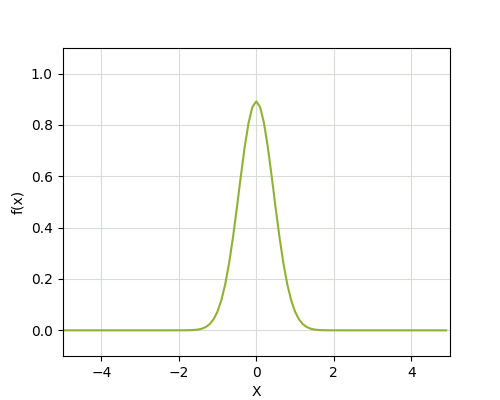
\includegraphics[width=.8\linewidth]{assets/normpdf00-02.png}
		\caption{Плотность вероятности}
		\label{fig:normpdf00-02}
	\end{subfigure}%
	\begin{subfigure}{.5\textwidth}
		\centering
		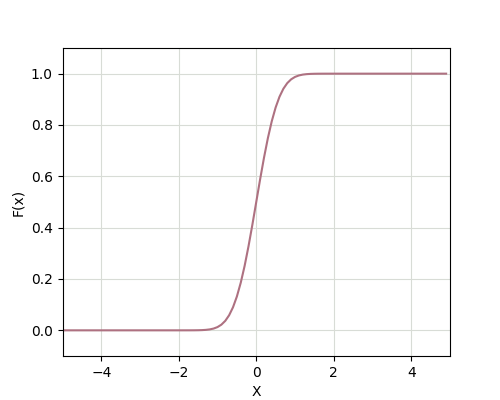
\includegraphics[width=.8\linewidth]{assets/normcdf00-02.png}
		\caption{Функция распределения}
		\label{fig:normcdf00-02}
	\end{subfigure}
	\caption{Нормальное распределение с параметрами $\mu = 0.0, \; \sigma^2 = 0.2$}
	\label{fig:norm00-02}
\end{figure}

\begin{figure}[H]
	\begin{subfigure}{.5\textwidth}
		\centering
		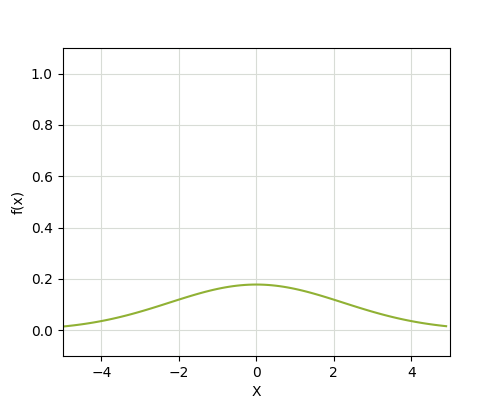
\includegraphics[width=.8\linewidth]{assets/normpdf00-50.png}
		\caption{Плотность вероятности}
		\label{fig:normpdf00-50}
	\end{subfigure}%
	\begin{subfigure}{.5\textwidth}
		\centering
		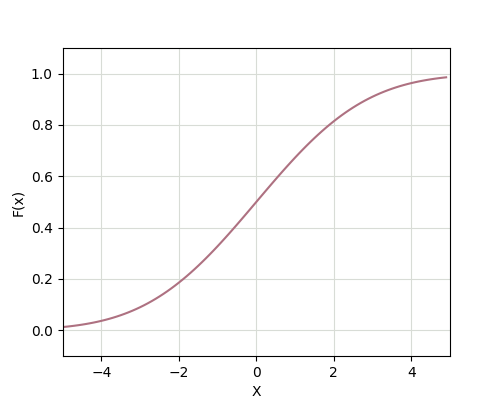
\includegraphics[width=.8\linewidth]{assets/normcdf00-50.png}
		\caption{Функция распределения}
		\label{fig:normcdf00-50}
	\end{subfigure}
	\caption{Нормальное распределение с параметрами $\mu = 0.0, \; \sigma^2 = 5.0$}
	\label{fig:norm00-50}
\end{figure}

\begin{figure}[H]
	\begin{subfigure}{.5\textwidth}
		\centering
		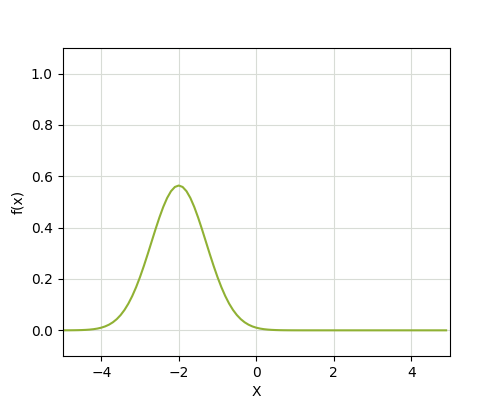
\includegraphics[width=.8\linewidth]{assets/normpdf-2-05.png}
		\caption{Плотность вероятности}
		\label{fig:normpdf-2-05}
	\end{subfigure}%
	\begin{subfigure}{.5\textwidth}
		\centering
		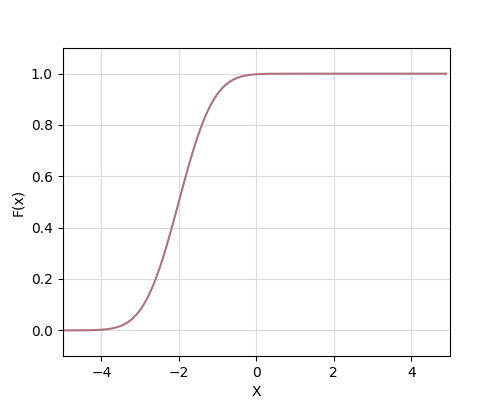
\includegraphics[width=.8\linewidth]{assets/normcdf-2-05.png}
		\caption{Функция распределения}
		\label{fig:normcdf-2-05}
	\end{subfigure}
	\caption{Нормальное распределение с параметрами $\mu = -2.0, \; \sigma^2 = 0.5$}
	\label{fig:norm-2-05}
\end{figure}

На рисунках \ref{fig:uni2-8} -- \ref{fig:uni-5-3} представлены полученные графики равномерного распределения с различными вариациями коэффициентов.
\begin{enumerate}
	\item Рисунок \ref{fig:uni2-8} -- $a = 2.0, \; b = 8.0$
	\item Рисунок \ref{fig:uni575-7} -- $a = 5.75, \; b = 7.0$
	\item Рисунок \ref{fig:uni-5-3} -- $a = -5.0, \; b = -3.0$
\end{enumerate}

\begin{figure}[H]
	\begin{subfigure}{.5\textwidth}
		\centering
		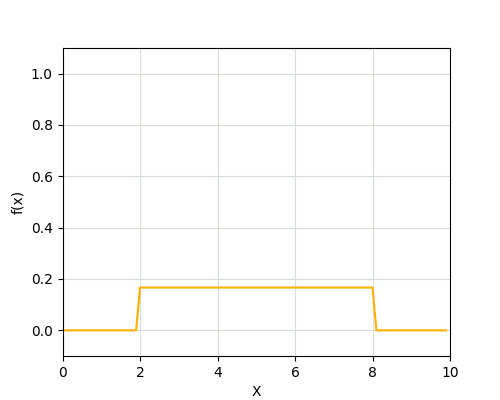
\includegraphics[width=.8\linewidth]{assets/unipdf2-8.png}
		\caption{Плотность вероятности}
		\label{fig:unipdf2-8}
	\end{subfigure}%
	\begin{subfigure}{.5\textwidth}
		\centering
		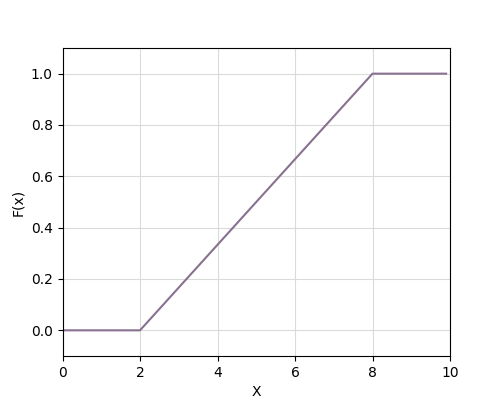
\includegraphics[width=.8\linewidth]{assets/unicdf2-8.png}
		\caption{Функция распределения}
		\label{fig:unicdf2-8}
	\end{subfigure}
	\caption{Равномерное распределение с параметрами $a = 2.0, \; b = 8.0$}
	\label{fig:uni2-8}
\end{figure}

\begin{figure}[H]
	\begin{subfigure}{.5\textwidth}
		\centering
		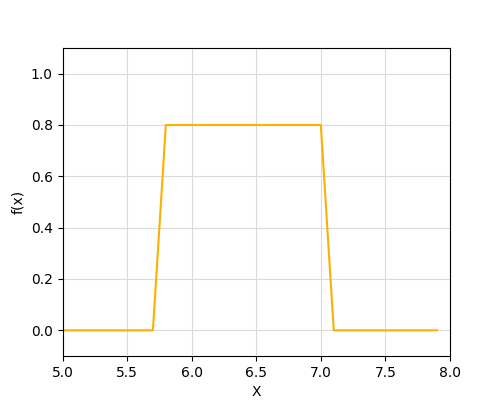
\includegraphics[width=.8\linewidth]{assets/unipdf575-7.png}
		\caption{Плотность вероятности}
		\label{fig:unipdf575-7}
	\end{subfigure}%
	\begin{subfigure}{.5\textwidth}
		\centering
		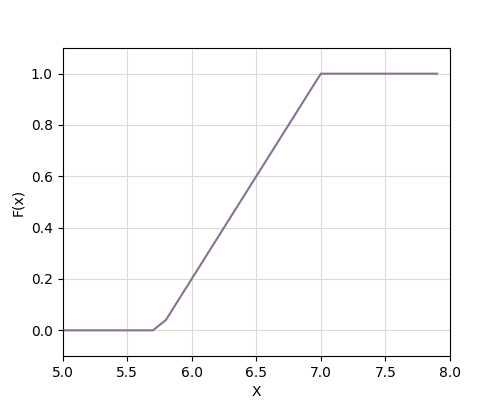
\includegraphics[width=.8\linewidth]{assets/unicdf575-7.png}
		\caption{Функция распределения}
		\label{fig:unicdf575-7}
	\end{subfigure}
	\caption{Равномерное распределение с параметрами $a = 5.75, \; b = 7.0$}
	\label{fig:uni575-7}
\end{figure}

\begin{figure}[H]
	\begin{subfigure}{.5\textwidth}
		\centering
		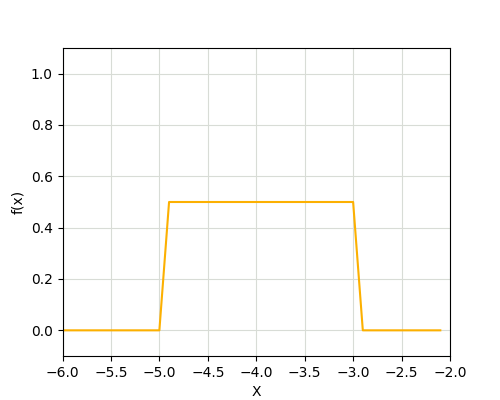
\includegraphics[width=.8\linewidth]{assets/unipdf-5-3.png}
		\caption{Плотность вероятности}
		\label{fig:unipdf-5-3}
	\end{subfigure}%
	\begin{subfigure}{.5\textwidth}
		\centering
		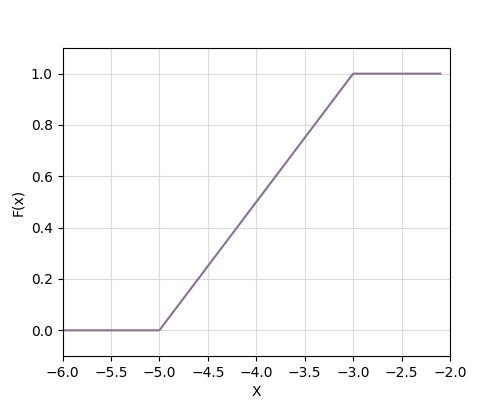
\includegraphics[width=.8\linewidth]{assets/unicdf-5-3.png}
		\caption{Функция распределения}
		\label{fig:unicdf-5-3}
	\end{subfigure}
	\caption{Равномерное распределение с параметрами $a = -5.0, \; b = -3.0$}
	\label{fig:uni-5-3}
\end{figure}
